\documentclass[a4paper,12pt]{article} % добавить leqno в [] для нумерации слева
\usepackage[a4paper,top=1.3cm,bottom=2cm,left=1.5cm,right=1.5cm,marginparwidth=0.75cm]{geometry}
%%% Работа с русским языком
\usepackage{cmap}					% поиск в PDF
\usepackage{mathtext} 				% русские буквы в фомулах
\usepackage[T2A]{fontenc}			% кодировка
\usepackage[utf8]{inputenc}			% кодировка исходного текста
\usepackage[english,russian]{babel}	% локализация и переносы

\usepackage{graphicx}

\usepackage{wrapfig}
\usepackage{tabularx}

\usepackage{hyperref}
\usepackage[rgb]{xcolor}
\hypersetup{
colorlinks=true,urlcolor=blue
}
\usepackage{multirow}
\usepackage{hhline}


%%% Дополнительная работа с математикой
\usepackage{amsmath,amsfonts,amssymb,amsthm,mathtools} % AMS
\usepackage{icomma} % "Умная" запятая: $0,2$ --- число, $0, 2$ --- перечисление

%% Номера формул
\mathtoolsset{showonlyrefs=true} % Показывать номера только у тех формул, на которые есть \eqref{} в тексте.

%% Шрифты
\usepackage{euscript}	 % Шрифт Евклид
\usepackage{mathrsfs} % Красивый матшрифт

%% Свои команды
\DeclareMathOperator{\sgn}{\mathop{sgn}}

%% Перенос знаков в формулах (по Львовскому)
\newcommand*{\hm}[1]{#1\nobreak\discretionary{}
{\hbox{$\mathsurround=0pt #1$}}{}}

\begin{document}
	
	\begin{titlepage}
	\begin{center}
		{\large МОСКОВСКИЙ ФИЗИКО-ТЕХНИЧЕСКИЙ ИНСТИТУТ (НАЦИОНАЛЬНЫЙ ИССЛЕДОВАТЕЛЬСКИЙ УНИВЕРСИТЕТ)}
	\end{center}
	\begin{center}
		{\large Физтех-школа электроники, фотоники и молекулярной физики}
	\end{center}
	
	
	\vspace{4.5cm}
	{\huge
		\begin{center}
			{Лабораторная работа 2.1.3}\\
			Определение $C_p/C_v$ по скорости звука в газе
		\end{center}
	}
	\vspace{2cm}
	\begin{flushright}
		{\LARGE Салтыкова Дарья \\
			\vspace{0.5cm}
			Б04-105}
	\end{flushright}
	\vspace{8cm}
	\begin{center}
		Долгопрудный 2022
	\end{center}
\end{titlepage}

\section{Введение}

\noindent
\textbf{Цель работы:} 1) измерение частоты колебаний и длины волны при резонансе звуковых колебаний в газе, заполняющем трубу; 2) определение показателя адиабаты с помощью уравнения состояния идеального газа.
\medskip

\noindent \textbf{Оборудование:} звуковой генератор ГЗ; электорнный осциллограф ЭО; микрофон; телефон; раздвижная труба; теплоизолированная труба, обогреваемая водой из термостата; баллон со сжатым углекислым газом; газгольдер.

\medskip

\section{Теоретические сведения}

\noindent Скорость распространения звуковой волны в газах зависит от показателя адиабаты $ \gamma $. На измерении скорости звука основан один из наиболее точных методов определения показателя адиабаты.

\medskip

\noindent Скорость звука в газах определяется формулой:

\begin{equation}\label{velocity}
c=\sqrt{\gamma\frac{RT}{\mu}}.
\end{equation}

\noindent где $ R $ -- газовая постоянная, $ T $ -- температура газа, а $ \mu $ -- его молярная масса. Преобразуя эту формулу, найдем

\begin{equation}
\gamma = \frac{\mu}{RT}c^2.
\end{equation}
\medskip

\noindent Таким образом, для определения показателя адиабаты достаточно измерить температуру газа и скорость распространения звука (молярная масса газа предполагается известной).

\medskip

\noindent Звуковая волна, распространяющаяся вдоль трубы, испытывает многократные отражения от торцов. Звуковые колебания в трубе являются наложением всех отраженных волн и очень сложны. Картина упрощается, если длина трубы $ L $ равна целому числу полуволн, то есть когда \[ L=n\lambda/2, \] где $ \lambda $ -- длина волны звука в трубе, а $ n $ -- любое целое число. Если это условие выполнено, то волна, отраженная от торца трубы, вернувшаяся к ее началу и вновь отраженная, совпадает по фазе с падающей. Совпадающие по фазе волны усиливают друг друга. Амплитуда звуковых колебаний при этом резко возрастает -- наступает резонанс.

\medskip

\noindent При звуковых колебаниях слои газа, прилегающие к торцам трубы, не испытывают смещения. Узлы смещения повторяются по всей длине трубы через $ \lambda/2 $. Между узлами находятся максимумы смещения.

\medskip

\noindent Скорость звука c связана с его частотой $ f $ и длиной волны $ \lambda $ соотношением

\begin{equation}\label{lambda_f}
c=\lambda f.
\end{equation}

\noindent Подбор условий, при которых возникает резонанс, можно производить двояко:
\begin{enumerate}

 \item При неизменной частоте $ f $ звукового генератора (а следовательно, и неизменной длине звуковой волны $ \lambda $) можно изменять длину трубы $ L $. Для этого применяется раздвижная труба. Длина раздвижной трубы постепенно увеличивается, и наблюдается ряд последовательных резонансов. Возникновение резонанса легко наблюдать на осциллографе по резкому увеличению амплитуды колебаний. Для последовательных резонансов имеем \begin{equation}
	\label{first}
	L_n=n\frac{\lambda}{2}, \quad L_{n+1}=(n+1)\frac{\lambda}{2}, \quad \dots, \quad L_{n+k} = n\frac{\lambda}{2}+k\frac{\lambda}{2},
	\end{equation} 
	
\noindent т. е. $ \lambda/2 $ равно угловому коэффициенту графика, изображающего зависимость длины трубы $ L $ от номера резонанса $ k $. Скорость звука находится по формуле \eqref{lambda_f}.

 \item При постоянной длине трубы можно изменять частоту звуковых колебаний. В этом случае следует плавно изменять частоту $ f $ звукового генератора, а следовательно, и длину звуковой волны $ \lambda $. Для последовательных резонансов получим 
	\begin{equation}\label{4}
	L=\frac{\lambda_1}{2}n=\frac{\lambda_2}{2}(n+1)=\dots=\frac{\lambda_{k+1}}{2}(n+k).
	\end{equation}
	
\noindent Из \eqref{lambda_f} и \eqref{4} имеем:
	\[ f_1=\frac{c}{\lambda_1}=\frac{c}{2L}n, \quad f_2=\frac{c}{\lambda_2}=\frac{c}{2L}(n+1)=f_1+\frac{c}{2L},\quad \dots, \]
	\begin{equation}\label{5}
	f_{k+1}=\frac{c}{\lambda_{k+1}}=\frac{c}{2L}(n+k)=f_1+\frac{c}{2L}k.
	\end{equation}
	
	\medskip
	
\noindent Скорость звука, деленная на $ 2L $, определяется, таким образом, по угловому коэффициенту графика зависимости частоты от номера резонанса.
\end{enumerate}


\section{Экспериментальная установка}

\noindent Соответственно двум методам измерения скорости звука в работе имеются две установки. В обеих установках звуковые колебания в трубе возбуждаются телефоном Т и улавливаются микрофоном М. Мембрана телефона приводится в движение переменным током звуковой частоты; в качестве источника переменной ЭДС используется звуковой генератор ГЗ. Возникающий в микрофоне сигнал наблюдается на осциллографе ЭО.

\medskip

\noindent Микрофон и телефон присоединены к установке через тонкие резиновые трубки. Такая связь достаточна для возбуждения и обнаружения звуковых колебаний в трубе и в то же время мало возмущает эти колебания: при расчетах оба торца трубы можно считать неподвижными, а влиянием соединительных отверстий пренебречь.

\medskip

\noindent Мы будем использовать первую установку (рис. 1), которая содержит раздвижную трубу с миллиметровой шкалой. Через патрубок (на рисунке не показан) труба может наполняться воздухом или углекислым газом из газгольдера. На этой установке производятся измерения $ \gamma $ для воздуха и для $ CO_2 $.
 
\begin{figure}[!h]
 	\centering
 	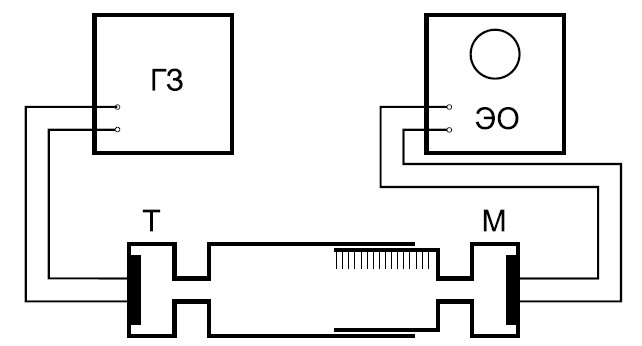
\includegraphics[width=0.6\linewidth]{установка.jpg}
 	\caption[]{Установка для измерения скорости звука при помощи раздвижной трубы}
 	
 \end{figure}
	
\newpage

\section{Ход работы}

\noindent Перепишем параметры установки:
$L = (700\pm5) \text{ мм},$  $\Delta L_{max} = (23 \pm1) \text{ мм}$
		
\medskip

\noindent Для проведения серии измерений фиксируем частоту звукового сигнала и оставляем её неизменной до окончания снятия показаний. Увеличиваем и уменьшаем длину трубки, чтобы добиться резонанса, возникновение которого устанавливается при помощи осциллографа. При возникновении резонанса фиксируем то расстояние $\Delta L$, на которое была выдвинута трубка прибора. Данные измерения проводим для нескольких значений частот. Полученные результаты заносим в таблицу.

\begin{table}[h!]
\begin{tabular}{|l|l|l|l|l|l|}
\hline
$f$,  кГц & 3,39 & 3,15 & 3,67 & 3,93 & 4,16 \\ \hline
$\Delta L$, см  & 0    & 0     & 0     & 0     & 0  \\ \cline{2-6} 
        & 5,3  & 5,7   & 5,0     & 4,3   & 4,1  \\ \cline{2-6} 
        & 10,4 & 11,2  & 9,5   & 8,7   & 8,3 \\ \cline{2-6} 
        & 15,5 & 16,6  & 14,2  & 13,1  & 12,4 \\ \cline{2-6} 
        & 20,7 & 22,2  & 19,0    & 17,5  & 16,6 \\ \cline{2-6} 
        &      &       &       & 21,9  &      \\ \hline
       
\end{tabular}
\end{table}


\noindent По полученным данным построим графики зависимости $ L(k) $, где k - номер резонанса (Рис.2)

\medskip
 
\noindent Угловой коэффициент наклона прямой $ a $ равен $ \lambda/2 $. Вычислим $ \lambda $ и результаты занесём в таблицу.

\medskip

\noindent Скорость звука в воздухе можно вычислить по следующей формуле: 
\[ c = \lambda f. \]

\noindent Погрешность такого вычисления равна \[ \sigma_c=c\sqrt{\varepsilon_f^2+\varepsilon_\lambda^2}. \] При этом в каждом измерении примем $ \sigma_f \approx 1 $ Гц.

\medskip

\begin{table}[h!]
\begin{tabular}{|l|l|l|l|l|l|l|}
\hline
f,  Гц & a, мм & $\sigma_a$, мм & $\lambda$, мм & $\sigma_\lambda$, мм & c, м/c  & $\sigma_c$, м/c \\ \hline
3390   & 51,6  & 0,2         & 103,2      & 0,4         & 349,8 & 1,4        \\ \hline
3150   & 55,3  & 0,3         & 110,6      & 0,6         & 348,4  & 1,9         \\ \hline
3670   & 47,2  & 0,4         & 94,4       & 0,8         & 346,4 & 2,9        \\ \hline
3930   & 43,8  & 0,08        & 87,6       & 0,16        & 344,3 & 0,6       \\ \hline
4160   & 41,5  & 0,1         & 83         & 0,2         & 345,3  & 0,8        \\ \hline
\end{tabular}
\end{table}

\noindent Усредняя вычисленные значения, в итоге получаем

$$ c_\text{возд} = (346,8 \pm 1,5) \text{ м/с}}\quad (\varepsilon=0,4\%) $$

\noindent Вычислим $ C_p/C_v $:

\[ \frac{C_p}{C_v} = \gamma = \frac{\mu}{RT}c^2. \]

\noindent При этом для воздуха $ \displaystyle \mu \approx 0,02898 \text{ } \frac{\text{кг}}{\text{моль}} $. Во время эксперимента температура в лаборатории равнялась $ T = (25,1 \pm 0,1) \text{ } ^\circ C $. Тогда погрешность такого вычисления можно оценить по следующей формуле:
$$\sigma_\gamma = \gamma\sqrt{\varepsilon_f^2+\left(2\varepsilon_c\right)^2}.$$

\noindent В итоге получаем:

$$\gamma_\text{возд} = 1,407
 \pm 0,009}\quad (\varepsilon=0,6\%)$$


\noindent Аналогичные измерения и вычисления проведем для углекислого газа. Перед началом измерений продуем трубу углекислым газом. Для этого при открытом
кране подвижную часть трубы следует несколько раз медленно выдвинуть
и затем резко вдвинуть в трубу. Графики зависимости L от k представлены на Рис.3.

\begin{table}[h!]
\begin{tabular}{|l|l|l|l|l|l|}
\hline
f,  кГц & 2,93 & 3,08 & 3,22 & 3,33 & 3,46 \\ \hline
dL, см  & -0,1 & -0,1 & -0,1 & -0,1 & -0,1 \\ \cline{2-6} 
        & 5,3  & 4,8  & 4,4  & 3,9  & 3,6  \\ \cline{2-6} 
        & 10,2 & 9,7  & 9    & 8,2  & 7,6  \\ \cline{2-6} 
        & 15   & 14,2 & 13,2 & 12,1 & 11,5 \\ \cline{2-6} 
        & 19,6 & 18,6 & 17,5 & 16,4 & 15,4 \\ \cline{2-6} 
        &      & 23   & 21,6 & 20,4 & 19,8 \\ \hline
\end{tabular}
\end{table}


\begin{table}[h!]
\begin{tabular}{|l|l|l|l|l|l|l|}
\hline
f,  Гц & a, мм & $\sigma_a$, мм & $\lambda$, мм & $\sigma_\lambda$, мм & c, м/c  & $\sigma_c$, м/c \\ \hline
2930   & 49,1  & 0,9         & 98,2       & 1,8         & 287,726 & 5,274        \\ \hline
3080   & 46,1  & 0,6         & 92,2       & 1,2         & 283,976 & 3,696        \\ \hline
3220   & 43,4  & 0,4         & 86,8       & 0,8         & 279,496 & 2,576        \\ \hline
3330   & 41,1  & 0,2         & 82,2       & 0,4         & 273,726 & 1,332        \\ \hline
3460   & 39,6  & 0,5         & 79,2       & 1           & 274,032 & 3,46         \\ \hline
\end{tabular}
\end{table}

$$ c_\text{CO}_2 = (279,8 \pm 3,2) \text{ м/с}}\quad (\varepsilon=1,2\%) $$

$$\gamma_\text{CO}_2 = 0,915
 \pm 0,015}\quad (\varepsilon=1,7\%)$$

\section{Вывод}

\medskip

\noindent В ходе работы были получены значения скорости звука и показателя адиабаты в воздухе углексилом газе. 

\medskip

\noindent Для воздуха получено:

$$ c_\text{возд} = (346,8 \pm 1,5) \text{ м/с}}\quad (\varepsilon=0,4\%) $$

$$\gamma_\text{возд} = 1,407
 \pm 0,009}\quad (\varepsilon=0,6\%)$$
 
\noindent Табличные значения (при T = 298 К): $ c_\text{табл} = 343 \text{ м/с, } \gamma_\text{табл} = 1,4$
 
\medskip 
 
\noindent Для углекислого газа получено:

$$ c_\text{CO}_2 = (279,8 \pm 3,2) \text{ м/с}}\quad (\varepsilon=1,2\%) $$

$$\gamma_\text{CO}_2 = 0,915
 \pm 0,015}\quad (\varepsilon=1,7\%)$$
 
\noindent Табличные значения (при нормальных условиях): $ c_\text{табл} = 259 \text{ м/с, } \gamma_\text{табл} = 1,3$

\medskip
\noindent Эксперементальные данные для воздуха в пределах погрешности соответствуют табличным. Для углекислого газа полченные значения отличатся от табличных, но по порядку величины совпадают.Вероятно, это связано с тем, что в трубе мог находиться углекислый газ с примесями (азот или кислород), которые могли исказить результаты измерений.
 
\section{Графики}

\begin{figure}[!h]
 	\centering
 	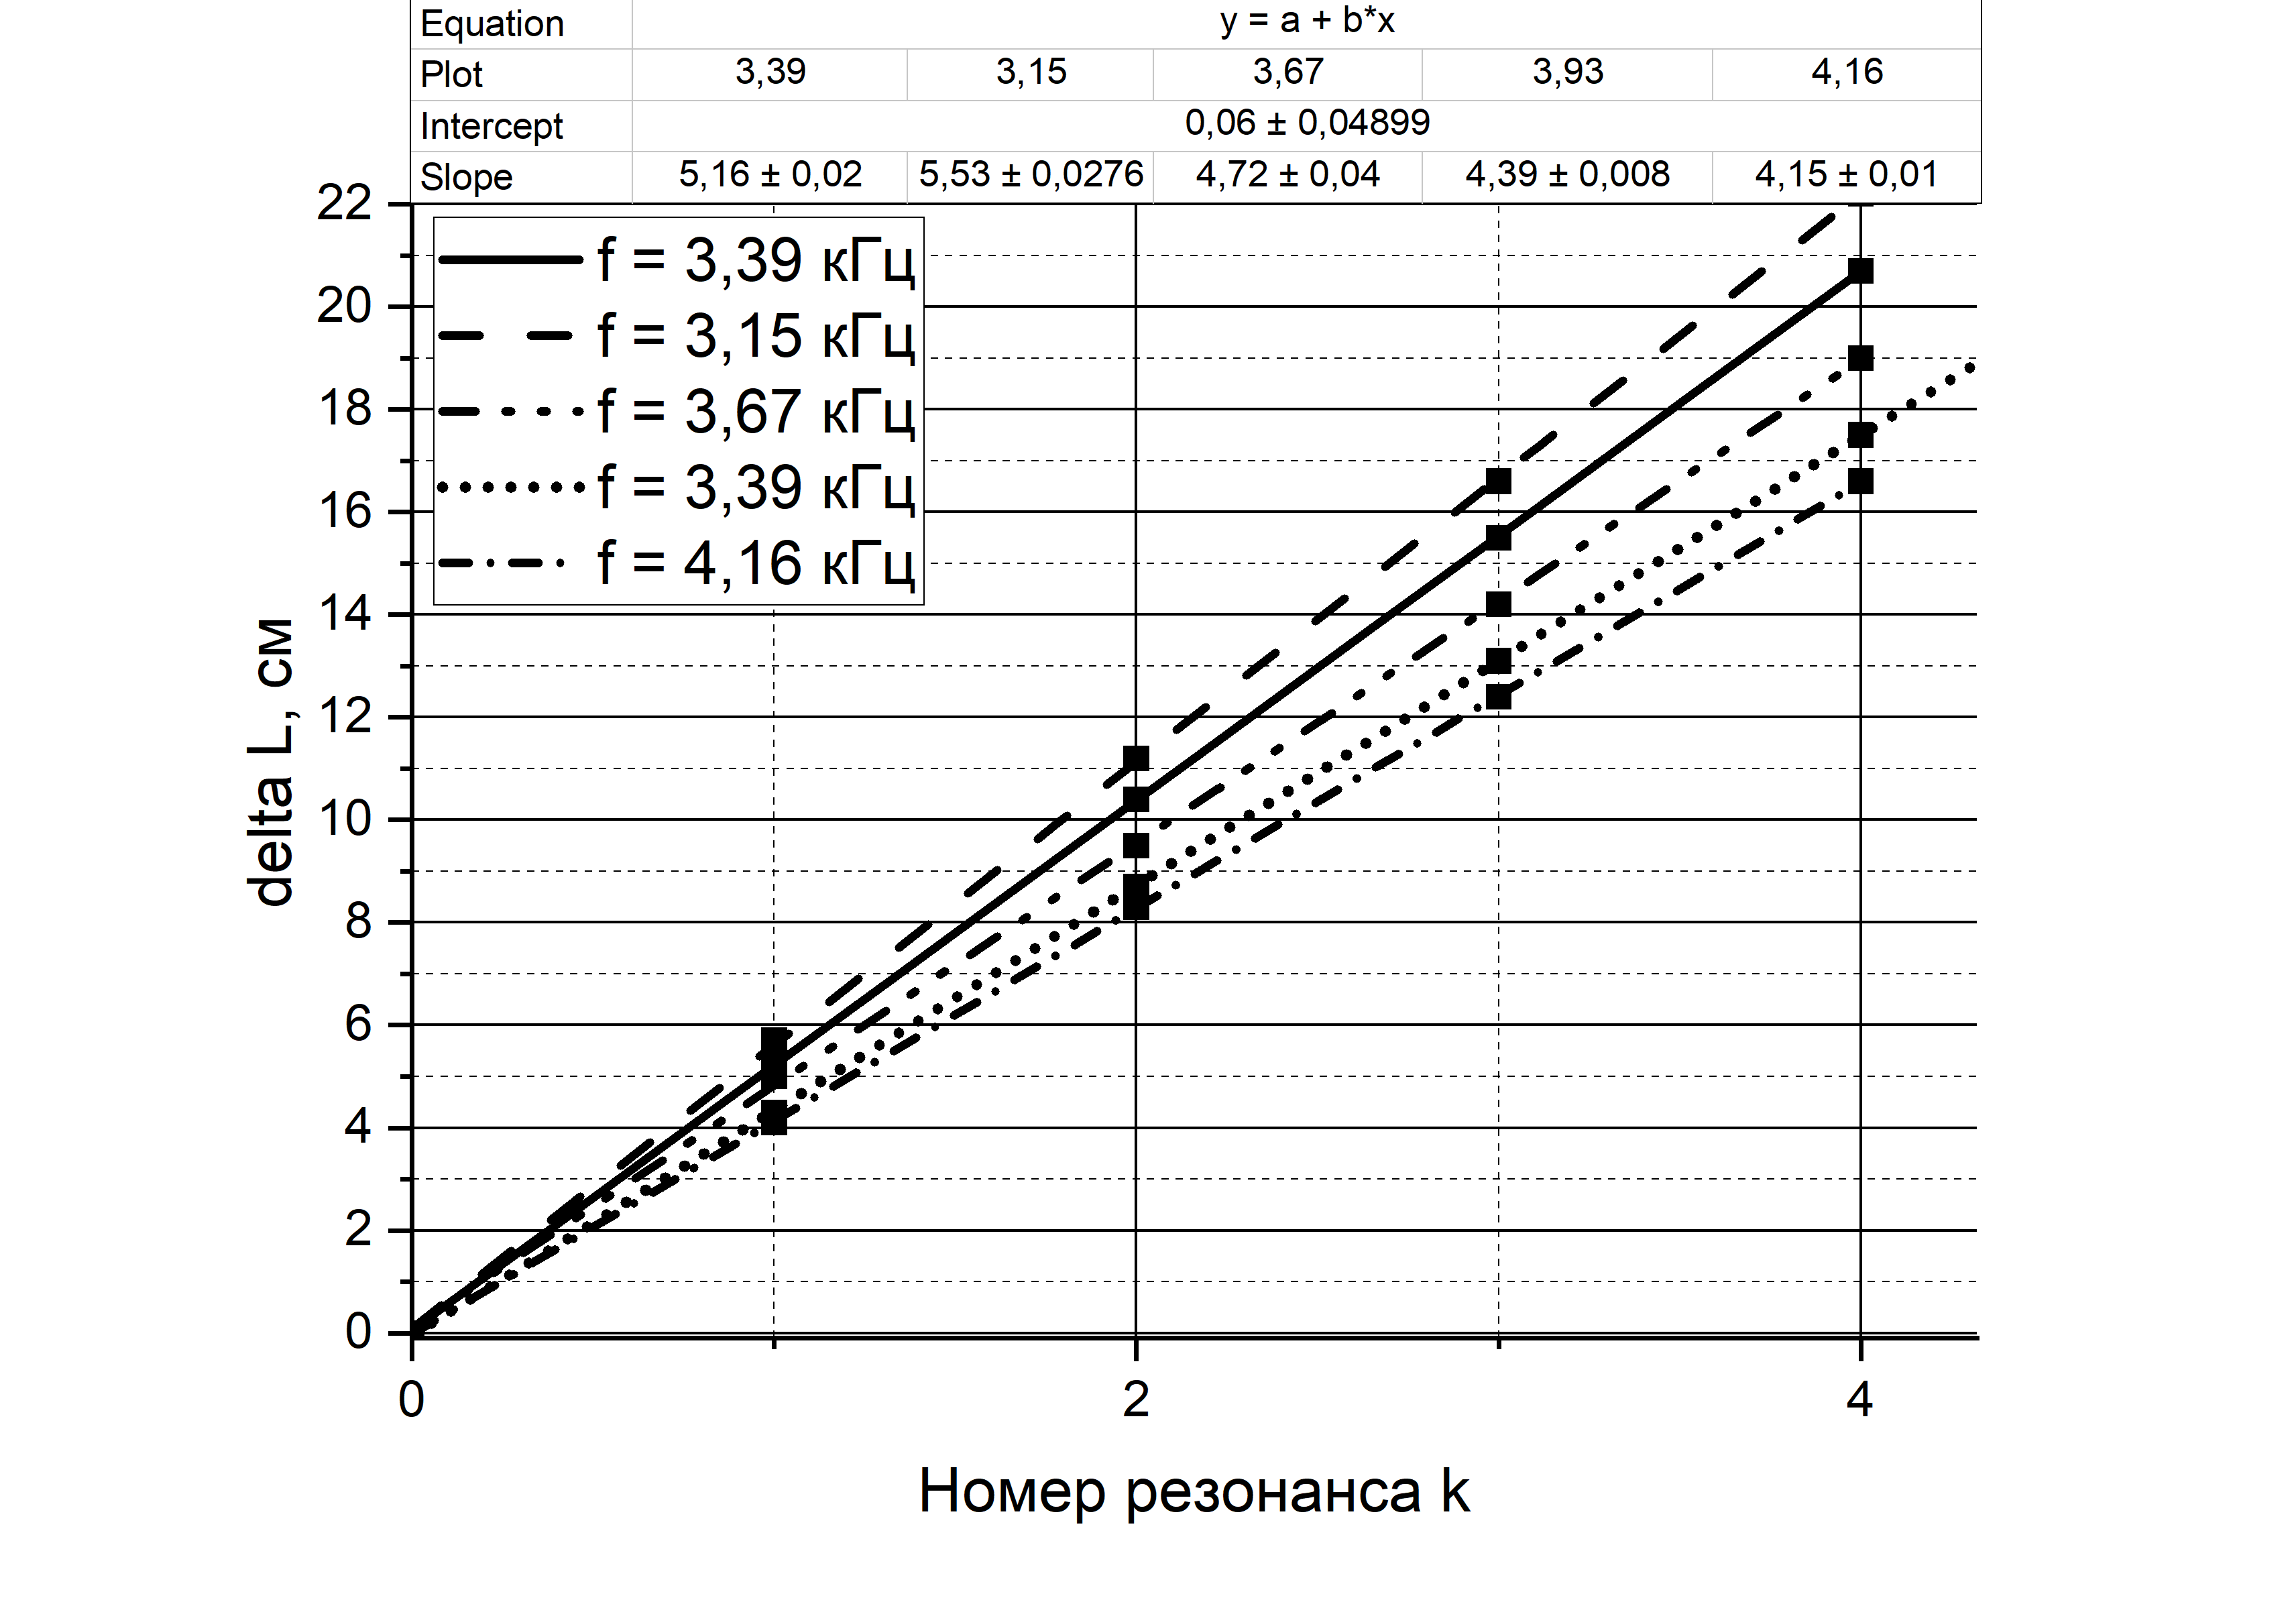
\includegraphics[width=1\linewidth]{воздух.png}
 	\caption[]{График зависимости L(k) для воздуха}
 
 \end{figure}
 
\begin{figure}[!h]
 	\centering
 	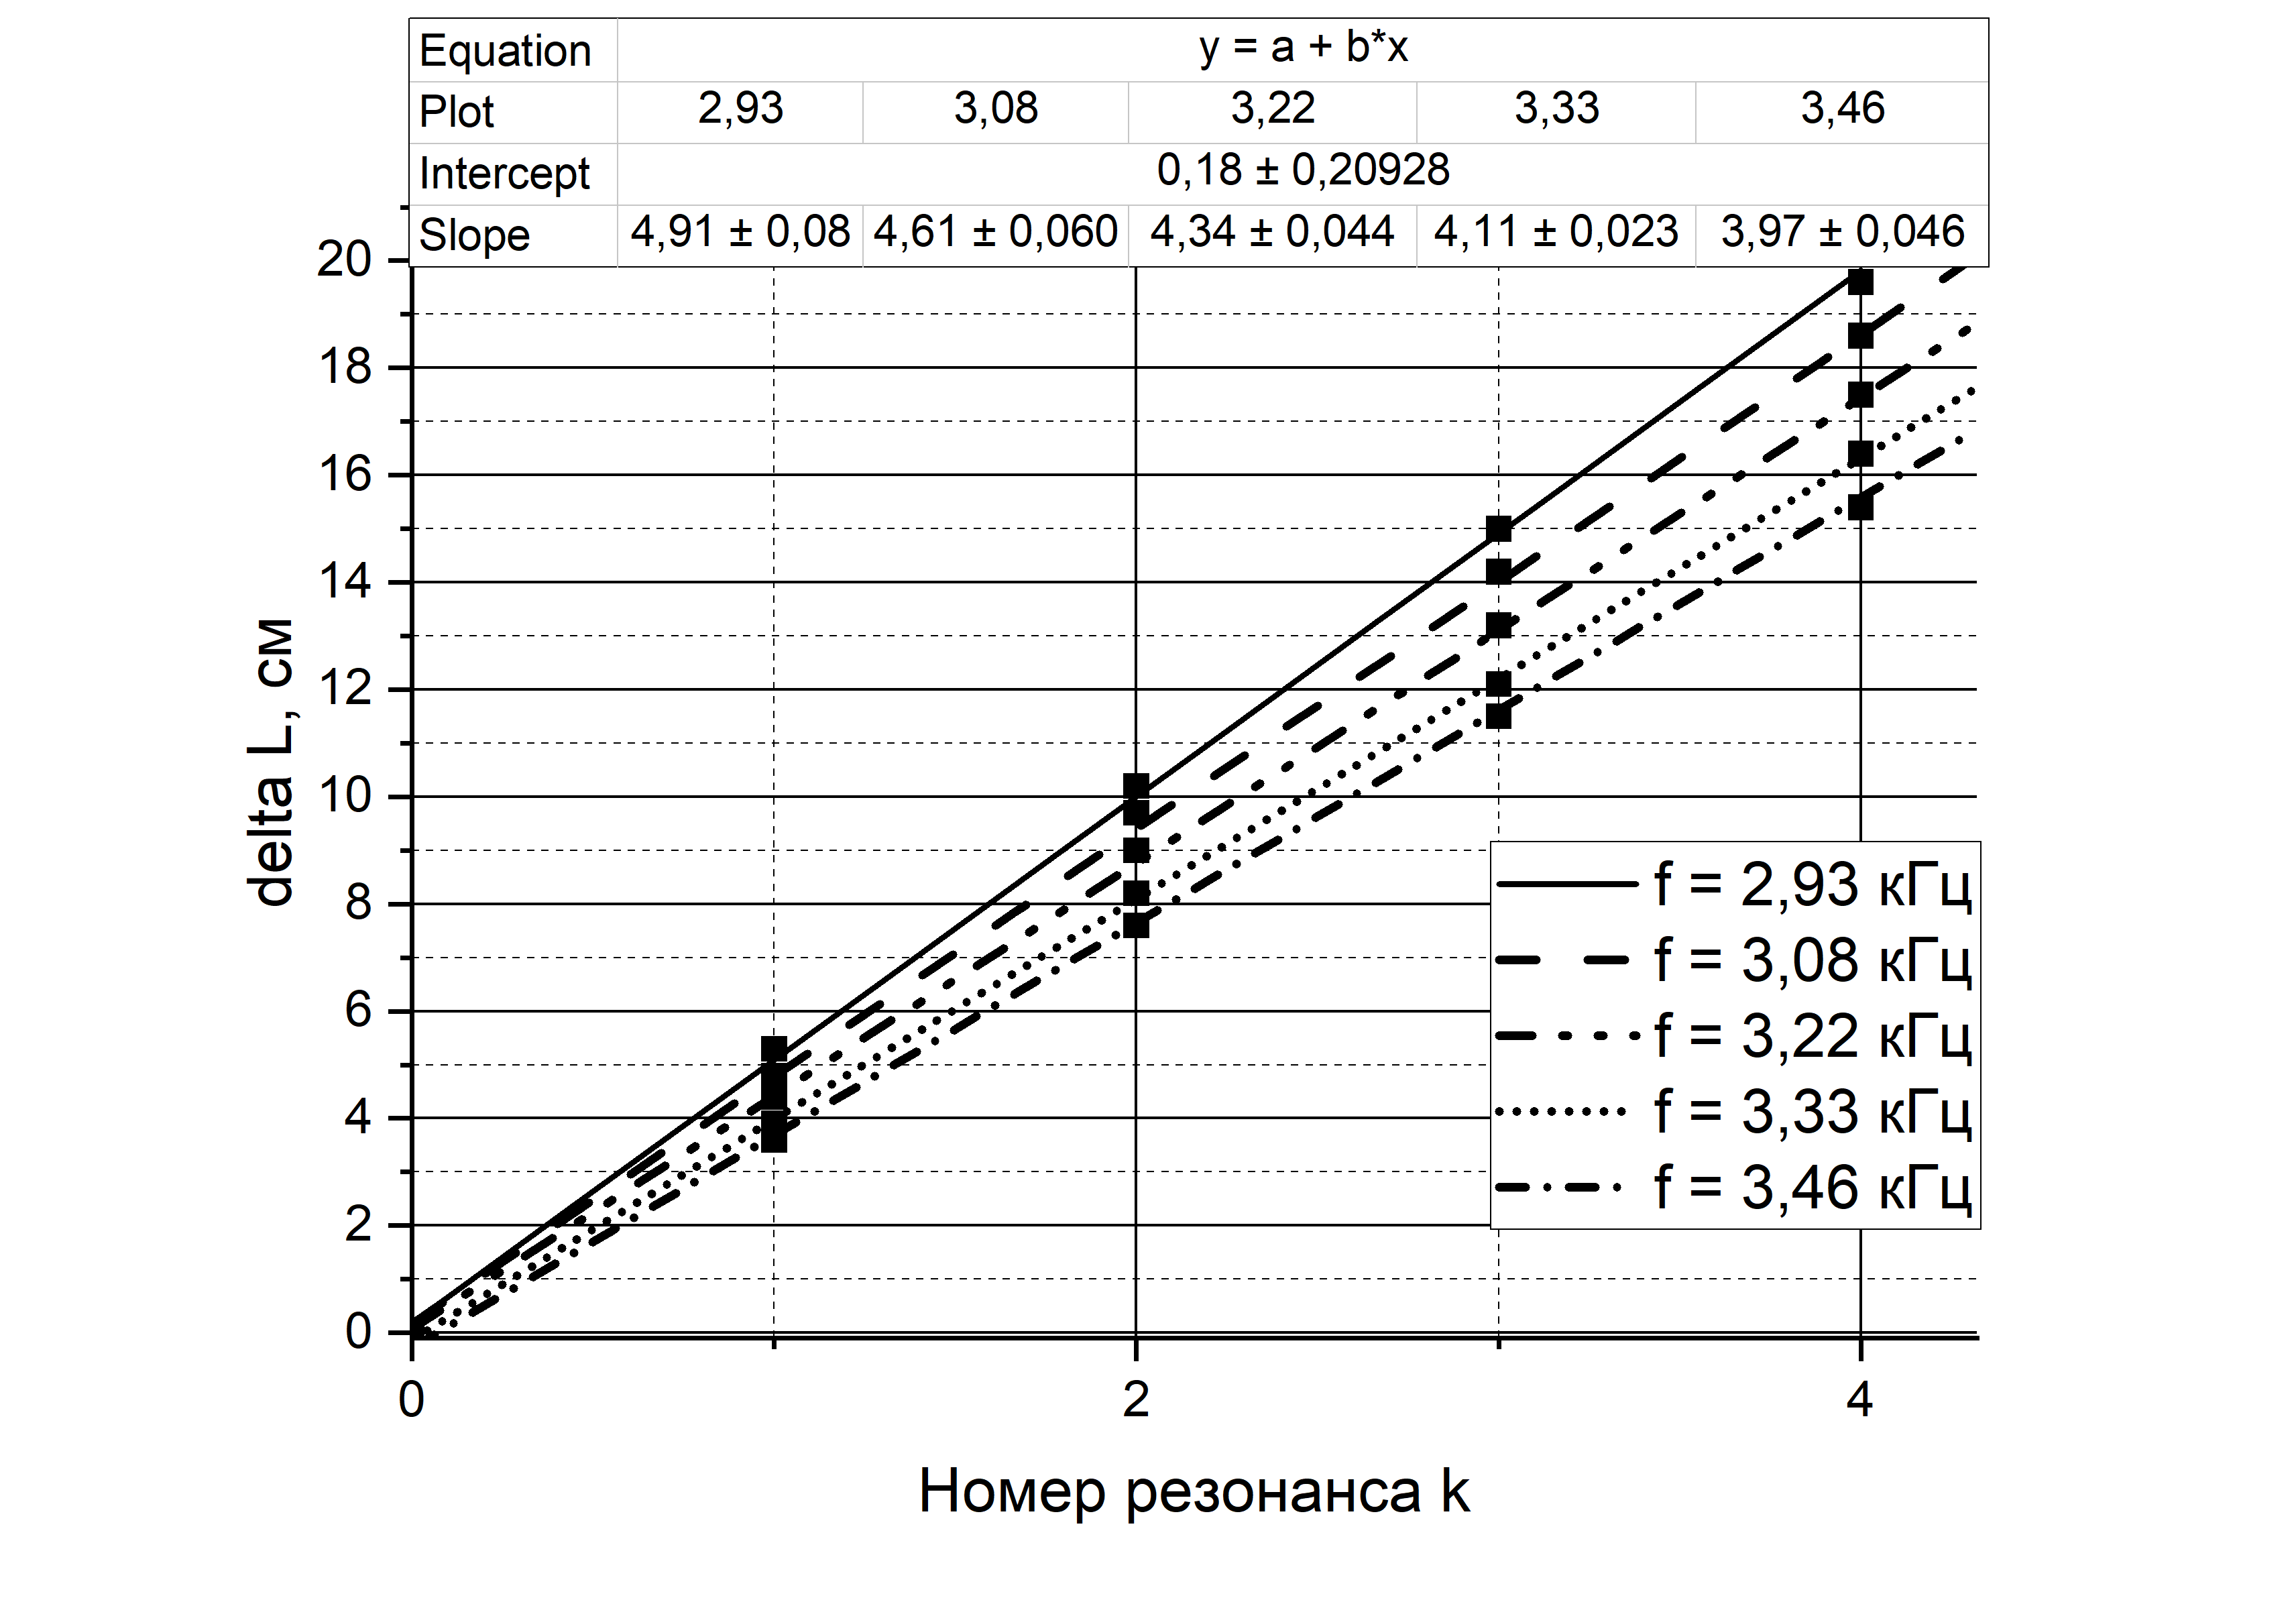
\includegraphics[width=1\linewidth]{CO2.png}
 	\caption[]{График зависимости L(k) для CO2}
 	
 \end{figure} 
 

\end{document}